\documentclass[journal, 11pt, onecolumn]{IEEEtran}
\usepackage{graphicx}
\usepackage{fancyhdr}
\usepackage{lastpage}
\usepackage[a4paper,margin=1in]{geometry}
\usepackage{newtxtext,newtxmath}
\usepackage{enumitem}
\usepackage{multicol}
\usepackage{array}

\usepackage{cite}
\usepackage{amsmath,amssymb,amsfonts,amsthm}
\usepackage{algorithmic}
\usepackage{graphicx}
\usepackage{textcomp}
\usepackage{xcolor}

\usepackage{listings}
\usepackage{enumitem}
\usepackage{mathtools}
\usepackage{gensymb}
\usepackage{comment}
\usepackage[breaklinks=true]{hyperref}
\usepackage{tkz-euclide} 
\usepackage{gvv}                                        
%\def\inputGnumericTable{}                                 
\usepackage[latin1]{inputenc}     
\usepackage{xparse}
\usepackage{color}                                            
\usepackage{array}                                            
\usepackage{longtable}                                       
\usepackage{calc}                                             
\usepackage{multirow}
\usepackage{multicol}
\usepackage{hhline}                                           
\usepackage{ifthen}                                           
\usepackage{lscape}
\usepackage{tabularx}
\usepackage{array}
\usepackage{float}
\newtheorem{theorem}{Theorem}[section]
\newtheorem{problem}{Problem}
\newtheorem{proposition}{Proposition}[section]
\newtheorem{lemma}{Lemma}[section]
\newtheorem{corollary}[theorem]{Corollary}
\newtheorem{example}{Example}[section]
\newtheorem{definition}[problem]{Definition}
\newcommand{\BEQA}{\begin{eqnarray}}
\newcommand{\EEQA}{\end{eqnarray}}
\newcommand{\define}{\stackrel{\triangle}{=}}
\theoremstyle{remark}
\newtheorem{rem}{Remark}

\graphicspath{{figs/}}


\pagestyle{fancy}

% Header and footer text
\fancyhead[L]{2012}
\fancyhead[C]{}
\fancyhead[R]{MAIN PAPER-MT}
\fancyfoot[L]{MT}
\fancyfoot[C]{}
\fancyfoot[R]{\thepage/\pageref{LastPage}}

% Adjust distances
\setlength{\headheight}{14pt}
\setlength{\headsep}{5pt}
\setlength{\footskip}{20pt}


% Line thickness
\renewcommand{\headrulewidth}{0.4pt}
\renewcommand{\footrulewidth}{0.4pt}

\begin{document}

\begin{center}
    \Large{AI25btech11020}
\end{center} 


\begin{enumerate}

\item A is a $2 \times 2$ matrix with $\det A = 2$. The $\det (2A)$ is
\begin{multicols}{4}
\begin{enumerate}  
\item 4
\item 8
\item 32
\item 16
\end{enumerate}
\end{multicols}
\hfill(GATE MT 2012)



\item A is a $2 \times 2$ matrix given below:
    \myvec{-3 & 1 \\-1 & -1}
The eigenvalues of $A$ are 
\begin{multicols}{4}
\begin{enumerate}  
\item $-2, -2$
\item $-3, -1$
\item $2, 2$
\item $3, 1$
\end{enumerate}
\end{multicols}
\hfill(GATE MT 2012)


\item In a production facility, iron rods are made with a mean diameter of 6 cm and standard deviation of 0.02 cm. If a large number of rods are tested, the approximate percentage of rods whose sizes fall in the range of 5.98 cm to 6.02 cm is
\begin{multicols}{4}
\begin{enumerate}  
\item 68
\item 75
\item 90
\item 99.7
\end{enumerate}
\end{multicols}
\hfill(GATE MT 2012)


\item Which one of the following methods is NOT used for numerical integration? 
\begin{multicols}{4}
\begin{enumerate}  
\item Rectangular rule
\item Trapezoidal rule
\item Simpson\textquotesingle s rule
\item Cramer\textquotesingle s rule
\end{enumerate}
\end{multicols}
\hfill(GATE MT 2012)
 

\item How many boundary conditions are required to solve the following equation?\\
\begin{center}
$\displaystyle \frac{\partial^2 T}{\partial r^2} 
+ \frac{1}{r} \frac{\partial T}{\partial r} 
= \frac{1}{\alpha} \frac{\partial T}{\partial t}$    
\end{center}

\begin{multicols}{2}
\begin{enumerate}  
\item Two in $r$-direction
\item One in $r$-direction and one for time
\item Two in $r$-direction and one for time
\item Three in $r$-direction and one for time
\end{enumerate}
\end{multicols}
\hfill(GATE MT 2012)
 

\item When a zinc metal rod is immersed in dilute hydrochloric acid, it results in 
\begin{multicols}{2}
\begin{enumerate}  
\item Evolution of hydrogen
\item Evolution of chlorine
\item Evolution of oxygen
\item No evolution of any gas
\end{enumerate}
\end{multicols}
\hfill(GATE MT 2012)

 

\item A fluid is flowing with a velocity of 0.5 m/s on a plate moving with a velocity of 0.01 m/s in the same direction. The velocity at the interface of the fluid and plate is  
\begin{multicols}{4}
\begin{enumerate}  
\item 0.0 m/s
\item 0.01 m/s
\item 0.255 m/s
\item 0.50 m/s
\end{enumerate}
\end{multicols}
\hfill(GATE MT 2012)
 

\item Hot metal at 1700 K is poured in a sand mould that is open at the top. Heat loss from the liquid metal takes place by 
\begin{multicols}{2}
\begin{enumerate}  
\item Radiation only
\item Radiation and conduction only
\item Radiation and convection only
\item Radiation, conduction and convection
\end{enumerate}
\end{multicols}
\hfill(GATE MT 2012)
 

\item Which one of the following is an equilibrium defect?
\begin{multicols}{4}
\begin{enumerate}  
\item Vacancies
\item Dislocations
\item Stacking faults
\item Grain boundaries
\end{enumerate}
\end{multicols}
\hfill(GATE MT 2012)

\item Floatation beneficiation is based on the principle of  
\begin{multicols}{2}
\begin{enumerate}  
\item Mineral surface hydrophobicity
\item Gravity difference
\item Chemical reactivity
\item Particle size difference
\end{enumerate}
\end{multicols}
\hfill(GATE MT 2012)
 

\item Copper can be reduced from acidic copper sulphate solution by  
\begin{multicols}{4}
\begin{enumerate}  
\item Silver
\item Iron
\item Carbon
\item Lead
\end{enumerate}
\end{multicols}
\hfill(GATE MT 2012)
 

\item Which one is NOT an agglomeration process?  
\begin{multicols}{4}
\begin{enumerate}  
\item Nodulizing
\item Briquetting
\item Roasting
\item Pelletizing
\end{enumerate}
\end{multicols}
\hfill(GATE MT 2012)
 

\item During LD blow in steelmaking the impurity that gets removed first is  
\begin{multicols}{4}
\begin{enumerate}  
\item Carbon
\item Phosphorous
\item Manganese
\item Silicon
\end{enumerate}
\end{multicols}
\hfill(GATE MT 2012)
 

\item During the solidification of a pure metal, it was found that dendrites are formed. Assuming that the liquid-solid interface is at the melting temperature, the temperature from the interface into the liquid  
\begin{multicols}{2}
\begin{enumerate}  
\item Decreases
\item Increases
\item Remains constant
\item Increases and then decreases
\end{enumerate}
\end{multicols}
\hfill(GATE MT 2012)
 

\item A peak in the X-ray diffraction pattern is observed at $2\theta = 78^\circ$, corresponding to $\{311\}$ planes of an fcc metal, when the incident beam has a wavelength of 0.154 nm. The lattice parameter of the metal is approximately  
\begin{multicols}{4}
\begin{enumerate}  
\item 0.6 nm
\item 0.4 nm
\item 0.3 nm
\item 0.2 nm
\end{enumerate}
\end{multicols}
\hfill(GATE MT 2012)
 

\item If $d$ is the inter-planar spacing of the planes $\{h k l\}$, the inter-planar spacing of the planes $\{n h n k n l\}$, $n$ being an integer, is  
\begin{multicols}{4}
\begin{enumerate}  
\item $d$
\item $d/n$
\item $nd$
\item $d/n^2$
\end{enumerate}
\end{multicols}
\hfill(GATE MT 2012)
 

\item As temperature increases, the electrical resistivities of pure metals ($\rho_m$) and intrinsic semiconductors ($\rho_s$) vary as follows  
\begin{multicols}{2}
\begin{enumerate}  
\item Both $\rho_m$ and $\rho_s$ increase
\item Both $\rho_m$ and $\rho_s$ decrease
\item $\rho_m$ increases and $\rho_s$ decreases
\item $\rho_m$ decreases and $\rho_s$ increases
\end{enumerate}
\end{multicols}
\hfill(GATE MT 2012)
 

\item At equilibrium spacing in a crystalline solid, which of the following is true for net inter-atomic force ($F$) and potential energy ($U$)  
\begin{multicols}{2}
\begin{enumerate}  
\item $F$ is zero and $U$ is zero
\item $F$ is zero and $U$ is minimum
\item $F$ is minimum and $U$ is zero
\item $F$ is minimum and $U$ is minimum
\end{enumerate}
\end{multicols}
\hfill(GATE MT 2012)
 

\item The property of a material that CANNOT be significantly changed by heat treatment is  
\begin{multicols}{2}
\begin{enumerate}  
\item Yield strength
\item Ultimate tensile strength
\item Ductility
\item Elastic modulus
\end{enumerate}
\end{multicols}
\hfill(GATE MT 2012)

\item A unit dislocation splits into two partial dislocations. The correct combination of the Burgers vectors of the partial dislocations for a given unit dislocation having Burgers vector \( \frac{a}{2}[\overline{1}10] \) is

\begin{multicols}{2}
\begin{enumerate}  
\item \( \frac{a}{6} [2\ \overline{1}\ 1] \) and \( \frac{a}{6} [1\ 2\ \overline{1}] \)
\item \( \frac{a}{6} [1\ \overline{1}\ 2] \) and \( \frac{a}{6} [\overline{1}\ 2\ 1] \)
\item \( \frac{a}{6} [1\ \overline{1}\ 2] \) and \( \frac{a}{6} [2\ 1\ \overline{1}] \)
\item \( \frac{a}{6} [2\ 1\ 1] \) and \( \frac{a}{6} [1\ 2\ \overline{1}] \)
\end{enumerate}
\end{multicols}
\hfill(GATE MT 2012)


\item A polymer matrix composite is reinforced with long continuous ceramic fibres aligned in one direction. The Young's moduli of the matrix and fibres are \(E_m\) and \(E_f\) respectively, and the volume fraction of the fibres is \(f\). Assuming iso-stress condition, Young's modulus of the composite \(E_c\) in a direction perpendicular to the length of fibres, is given by the expression

\begin{multicols}{2}
\begin{enumerate}  
\item \( E_c = (1-f)E_m + f E_f \)
\item \( E_c = fE_m + (1-f)E_f \)
\item \( \frac{1}{E_c} = \frac{(1-f)}{E_m} + \frac{f}{E_f} \)
\item \( \frac{1}{E_c} = \frac{f}{E_m} + \frac{(1-f)}{E_f} \)
\end{enumerate}
\end{multicols}
\hfill(GATE MT 2012)

\item Which of the following is NOT a fusion welding process?

\begin{multicols}{2}
\begin{enumerate}  
\item Arc welding
\item Gas welding
\item Resistance welding
\item Friction stir welding
\end{enumerate}
\end{multicols}
\hfill(GATE MT 2012)

\item Tungsten filament used in electric bulb is processed by

\begin{multicols}{2}
\begin{enumerate}  
\item Extrusion
\item Wire drawing
\item Casting
\item Powder metallurgy
\end{enumerate}
\end{multicols}
\hfill(GATE MT 2012)

\item The riser is designed such that the melt in the riser solidifies

\begin{enumerate}  
\item Before casting solidifies
\item At the same time as casting solidifies
\item After casting solidifies
\item Irrespective of the solidification of the casting
\end{enumerate}
\hfill(GATE MT 2012)


\item Radiography technique of detecting defects is based on the principle of

\begin{multicols}{4}
\begin{enumerate}  
\item Diffraction
\item Reflection
\item Interference
\item Absorption
\end{enumerate}
\end{multicols}
\hfill(GATE MT 2012)

\item At \(x=0.5\), the polynomial \(x^2(1-x^2)\) has

\begin{multicols}{4}
\begin{enumerate}  
\item No extrema
\item A saddle point
\item A minima
\item A maxima
\end{enumerate}
\end{multicols}
\hfill(GATE MT 2012)

\item Given that $\mathbf{v}$ is a vector field and $f$ is a scalar field, match the equations in \textbf{Group I} with their physical meaning in \textbf{Group II}
\begin{multicols}{2}
\underline{Group 1}
\begin{enumerate}[label=(\Alph*), start=16]
\item $\mathrm{div}\ (\mathbf{v}) = 0$  
\item $\mathrm{curl}\ (\mathrm{grad}(f)) = 0$
\item $\mathrm{div}\ (\mathrm{grad}(f)) = 0$
\item $\mathbf{v} = \mathrm{grad}(f)$
\end{enumerate}

\underline{Group 2}
\begin{enumerate}[label=(\arabic*), start=1]
\item Irrotational 
\item Incompressible
\item Potential
\item Laplace equation 
\end{enumerate}
\end{multicols}

\begin{multicols}{2}
\begin{enumerate}  
\item P-1, Q-2, R-3, S-4
\item P-2, Q-1, R-4, S-3
\item P-1, Q-3, R-2, S-4
\item P-2, Q-1, R-3, S-4
\end{enumerate}
\end{multicols}
\hfill(GATE MT 2012)

\item The temperature field of a slab is given by $T = 400 - 50z \exp(-t - x^2 - y^2)$. The temperature gradient in $y$-direction is

\begin{multicols}{2}
\begin{enumerate}  
\item $100yz \exp(-t - x^2 - y^2)$
\item $-100yz \exp(-t - x^2 - y^2)$
\item $100xz \exp(-t - x^2 - y^2)$
\item $-100xz \exp(-t - x^2 - y^2)$
\end{enumerate}
\end{multicols}
\hfill(GATE MT 2012)

% Q.29
\item What does the solution of the following ordinary differential equation represent? 
\begin{align}
    y \frac{dy}{dx} + x = 0
\end{align}

\begin{multicols}{2}
\begin{enumerate}  
\item A parabola
\item A circle
\item An ellipse
\item A hyperbola
\end{enumerate}
\end{multicols}
\hfill(GATE MT 2012)

% Q.30
\item A thin layer of material B (of total amount $m$) is plated on the end faces of two long rods of material A. These are then joined together on the plated side (see the figure below) and heated to a high temperature. Assuming the diffusion coefficient of B in A is $D$, the composition profile $c_B$ along the rod axis $x$ after a time $t$ is described by

\begin{figure}
    \centering
    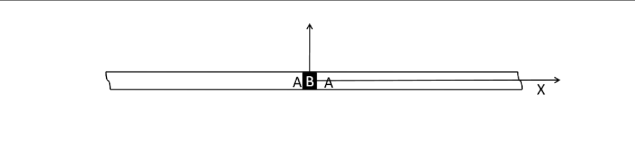
\includegraphics[width=0.5\linewidth]{figs/a5f1.png}
    
    \caption{}
    \label{fig:placeholder}
\end{figure}

\begin{multicols}{2}
\begin{enumerate}  
\item $c_B = \dfrac{m}{2\sqrt{\pi D t}} \exp \left[ - \dfrac{x^2}{4Dt} \right]$
\item $c_B = \dfrac{m}{2\sqrt{\pi D t}} \mathrm{erf} \left[ - \dfrac{x^2}{4Dt} \right]$
\item $c_B = \dfrac{m}{2\sqrt{\pi D t}} \left[ 1 - \mathrm{erf} \left( - \dfrac{x^2}{4Dt} \right)\right]$
\item $c_B = \dfrac{m}{2\sqrt{\pi D t}} t$
\end{enumerate}
\end{multicols}
\hfill(GATE MT 2012)

\item Match the principles given in \textbf{Group I} with corresponding corrosion terminology in \textbf{Group II}

\begin{multicols}{2}
\underline{Group 1}
\begin{enumerate}[label=(\Alph*), start=16]
\item Electrode polarization  
\item Passivity 
\item Selective leaching
\item Grain boundary precipitation
\end{enumerate}

\underline{Group 2}
\begin{enumerate}[label=(\arabic*), start=1]
\item Dezinfication
\item Intergranular attack 
\item Over voltage
\item Surface oxide film 
\end{enumerate}
\end{multicols}

\begin{multicols}{2}
\begin{enumerate}  
\item P-3, Q-4, R-1, S-2
\item P-3, Q-4, R-2, S-1
\item P-4, Q-2, R-1, S-3
\item P-2, Q-1, R-4, S-3
\end{enumerate}
\end{multicols}
\hfill(GATE MT 2012)

% Q.32
\item Identify the correct combination of the following statements

P. Hydrogen electrode is a standard used to measure redox potentials \\
Q. Activation polarization refers to electrochemical processes controlled by reaction sequence at metal-solution interface \\
R. Potential-pH diagrams can be used to predict corrosion rates of metals \\
S. Cathodic protection can use sacrificial anodes such as magnesium

\begin{multicols}{2}
\begin{enumerate}  
\item P, Q and R
\item Q, R and S
\item P, Q and S
\item P, R and S
\end{enumerate}
\end{multicols}
\hfill(GATE MT 2012)

% Q.33
\item Consider a reaction with activation energy of 8.314 kJ/mol that takes place at 300 K. If the reaction rate is to be tripled, the temperature of the reaction should be

\begin{multicols}{2}
\begin{enumerate}  
\item 174.5 K
\item 447.5 K
\item 600.5 K
\item 847.5 K
\end{enumerate}
\end{multicols}
\hfill(GATE MT 2012)

% Q.34
\item Match the processes in \textbf{Group I} with the objectives in \textbf{Group II}
\begin{multicols}{2}
\underline{Group 1}
\begin{enumerate}[label=(\Alph*), start=16]
\item Vacuum Arc Degassing (VAD)  
\item LD
\item COREX 
\item Blast Furnace
\end{enumerate}

\underline{Group 2}
\begin{enumerate}[label=(\arabic*), start=1]
\item Primary iron making 
\item Secondary steel making 
\item Direct smelting
\item Primary steel making 
\end{enumerate}
\end{multicols}

\begin{multicols}{2}
\begin{enumerate}
\item P-3, Q-4, R-2, S-1
\item P-4, Q-3, R-1, S-2
\item P-3, Q-2, R-1, S-4
\item P-2, Q-4, R-3, S-1
\end{enumerate}
\end{multicols}
\hfill(GATE MT 2012)

\item The reduction of FeO with CO gas in co-current flow is given by the following equation: \\
\[
    \text{FeO} + \text{CO} = \text{Fe} + \text{CO}_2 \qquad \Delta G^\circ = 8120 \text{ J at 1173 K}
\]
The ratio of $P_{CO}/P_{CO_2}$ for this reaction at $1173$ K is

\begin{multicols}{2}
\begin{enumerate}  
\item 0.0
\item 0.25
\item 0.44
\item 2.3
\end{enumerate}
\end{multicols}
\hfill(GATE MT 2012)

\item The sulphide capacity ($C_S$) of liquid slag of composition 55 wt.\% CaO, 20 wt.\% SiO$_2$, 15 wt.\% Al$_2$O$_3$, and 10 wt.\% MgO is given by the following equation \\
\[
    \log C_S = -3.44 \, (X_{CaO} + 0.1 X_{MgO} - 0.8 X_{Al_2O_3} - X_{SiO_2}) - \frac{9894}{T} + 2.05
\]
where, $X$ is mole fraction of the respective components. Atomic weights of Ca, Mg, Si, Al and O are 40, 24, 28, 27 and 16 respectively. \\
The value of $C_S$ at $1900$ K is
\begin{multicols}{2}
\begin{enumerate}  
\item 0.0009
\item 0.009
\item 0.09
\item 0.9
\end{enumerate}
\end{multicols}
\hfill(GATE MT 2012)

\item Match the processes given in \textbf{Group I} with the corresponding metals in \textbf{Group II}
\begin{multicols}{2}
\underline{Group 1}
\begin{enumerate}[label=(\Alph*), start=16]
\item Matte smelting   
\item Cyanide leaching
\item Carbothermic reduction 
\item Fused salt electrolysis
\end{enumerate}
\hfill(GATE MT 2012)

\underline{Group 2}
\begin{enumerate}[label=(\arabic*), start=1]
\item Lead 
\item Copper
\item Aluminium
\item Gold
\end{enumerate}
\end{multicols}

\begin{multicols}{2}
\begin{enumerate}
\item P-1, Q-2, R-1, S-4
\item P-2, Q-3, R-1, S-4
\item P-2, Q-1, R-3, S-4
\item P-2, Q-3, R-4, S-1
\end{enumerate}
\end{multicols}
\hfill(GATE MT 2012)

\item Identify the correct combination of the following statements

P. Bessemer converter can be used in copper smelting \\
Q. The Mond process for nickel involves reaction of metal with H$_2$ gas \\
R. Roasted ZnS concentrates can be smelted in a blast furnace \\
S. Magnesium metal can be produced by electrolysis of sea water

\begin{multicols}{2}
\begin{enumerate}  
\item P, R and S
\item P, Q and R
\item P and Q
\item Q and S
\end{enumerate}
\end{multicols}
\hfill(GATE MT 2012)

\item Match the phases of steel in \textbf{Group I} with the crystal structures in \textbf{Group II}
\begin{multicols}{2}
\underline{Group 1}
\begin{enumerate}[label=(\Alph*), start=16]
\item Martensite   
\item Cementite
\item Austenite  
\item Ferrite
\end{enumerate}

\underline{Group 2}
\begin{enumerate}[label=(\arabic*), start=1]
\item bcc 
\item fcc
\item bct
\item Orthorhombic
\end{enumerate}
\end{multicols}

\begin{multicols}{2}
\begin{enumerate}  
\item P-3, Q-4, R-1, S-2
\item P-2, Q-3, R-1, S-4
\item P-3, Q-4, R-2, S-1
\item P-4, Q-3, R-2, S-1
\end{enumerate}
\end{multicols}
\hfill(GATE MT 2012)

\item Arrange the following in terms of increasing severity of quench

P. Oil quenching \\
Q. Water quenching \\
R. Water quenching with agitation \\
S. Brine quenching

\begin{multicols}{2}
\begin{enumerate}  
\item P<Q<R<S
\item Q<R<P<S
\item P<Q<S<R
\item Q<P<R<S
\end{enumerate}
\end{multicols}
\hfill(GATE MT 2012)

\item Regarding recrystallization, which one of the following statements is NOT correct?

\begin{enumerate}  
\item Higher the amount of cold work, lower is the recrystallization temperature
\item Higher the recovery, higher is the recrystallization temperature
\item Higher the temperature of cold work, higher is the recrystallization temperature
\item Finer the initial grain size, higher is the recrystallization temperature
\end{enumerate}
\hfill(GATE MT 2012)

\item A liquid droplet ($\beta$) is on a substrate ($\delta$) and is surrounded by air ($\alpha$), as shown below. The angle of contact ($\theta$) is determined using the following expression:

\begin{figure}
    \centering
    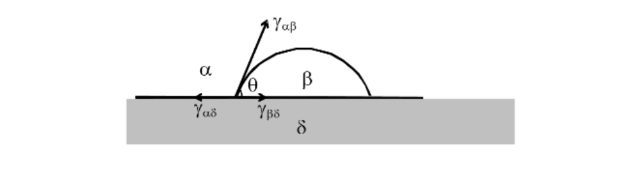
\includegraphics[width=0.5\linewidth]{figs/a5f2.png}
    \caption{}
    \label{fig:placeholder}
\end{figure}

\begin{multicols}{2}
\begin{enumerate}  
\item $\theta = \cos^{-1} \left( \dfrac{\gamma_{\alpha \delta} - \gamma_{\beta \delta}}{\gamma_{\alpha \beta}} \right)$
\item $\theta = \cos^{-1} \left( \dfrac{\gamma_{\delta \delta} - \gamma_{\alpha \beta}}{\gamma_{\alpha \beta}} \right)$
\item $0 = \cos^{-1} \left( \dfrac{\gamma_{\alpha \delta} - \gamma_{\beta \delta}}{\gamma_{\alpha \delta}} \right)$
\item $\theta = \cos^{-1} \left( \dfrac{\gamma_{\alpha \delta} - \gamma_{\beta \delta}}{\gamma_{\beta \delta}} \right)$
\end{enumerate}
\end{multicols}
\hfill(GATE MT 2012)

\item Match the phenomena listed in \textbf{Group I} with the possible mechanisms in \textbf{Group II}
\begin{multicols}{2}
\underline{Group 1}
\begin{enumerate}[label=(\Alph*), start=16]
\item Fatigue   
\item Creep
\item Strain hardening  
\item Yield point phenomenon
\end{enumerate}

\underline{Group 2}
\begin{enumerate}[label=(\arabic*), start=1]
\item Grain boundary sliding 
\item Slip band extrusion and intrusion
\item Cottrell atmosphere
\item Dislocation interaction
\end{enumerate}
\end{multicols}

\begin{multicols}{2}
\begin{enumerate}  
\item P-2, Q-3, R-4, S-1
\item P-2, Q-4, R-3, S-1
\item P-1, Q-2, R-4, S-3
\item P-1, Q-2, R-4, S-3
\end{enumerate}
\end{multicols}
\hfill(GATE MT 2012)

% Q.44
\item Fracture stress for a brittle material having a crack length of 1 $\mu$m is 200 MPa. Fracture stress for the same material having a crack length of 4 $\mu$m is
\begin{multicols}{2}
\begin{enumerate}  
\item 200 MPa
\item 150 MPa
\item 100 MPa
\item 50 MPa
\end{enumerate}
\end{multicols}
\hfill(GATE MT 2012)

% Q.45
\item The flow stress ($\overline{\sigma}$) of an alloy varies with strain rate ($\dot{\epsilon}$) as $\overline{\sigma} = 100(\dot{\epsilon})^{0.1}$ MPa. When the alloy is hot extruded from 10 cm diameter to 5 cm diameter at a speed of 2 cm/s, the flow stress is
\begin{multicols}{2}
\begin{enumerate}  
\item 1000 MPa
\item 105 MPa
\item 150 MPa
\item 1050 MPa
\end{enumerate}
\end{multicols}
\hfill(GATE MT 2012)

% Q.46
\item Determine the correctness or otherwise of the following \textbf{Assertion (a)} and \textbf{Reason (r)}.
\\[0.5em]\textit{Assertion}: During rolling, front tension and (or) back tension are (is) employed to decrease rolling load.\\
\textit{Reason}: Roll pressure decreases due to lowering of flow stress as a result of front tension/back tension.
\begin{enumerate}  
\item A is false but R is true
\item A is true and R is also true, but r is not the reason for a
\item A is true and R is also true, and r is the reason for a
\item A is true but R is false
\end{enumerate}
\hfill(GATE MT 2012)


\item Match the defects listed in \textbf{Group I} with the processes listed in \textbf{Group II}

\begin{multicols}{2}
\underline{Group 1}
\begin{enumerate}[label=(\Alph*), start=16]
\item Cold shut  
\item Earing
\item Alligatoring  
\item Shrinkage porosity
\end{enumerate}

\underline{Group 2}
\begin{enumerate}[label=(\arabic*), start=1]
\item Rolling 
\item Forging 
\item Deep drawing
\item Fusion welding
\end{enumerate}
\end{multicols}

\begin{multicols}{2}
\begin{enumerate}
\item P-2, Q-4, R-1, S-4
\item P-2, Q-4, R-3, S-1
\item P-2, Q-3, R-1, S-4
\item P-4, Q-1, R-2, S-3
\end{enumerate}
\end{multicols}
\hfill(GATE MT 2012)

\item[] \textbf{Common Data for Questions 48 and 49:} \\
A steel ball (density $\rho_{steel}=7200$kg/m$^3$) is placed in an upward moving liquid Al (density $\rho_{Al}=2360$kg/m$^3$, viscosity $\mu_{Al}=1\times10^3$ Pa.s and Reynolds number $=5\times10^5$). The force ($F$) exerted on the steel ball is expressed as \\
\[
    F = f \pi R^2 \left( \rho_{Al}v^2/2 \right)
\]
where $f$ is friction factor (=0.2), $v$ is the velocity of liquid Al and $R$ is the radius of steel ball.

\item The force exerted on the steel ball is
\begin{multicols}{2}
\begin{enumerate}  
\item 8.32 N
\item 6.70 N
\item 1.67 N
\item 0.52 N
\end{enumerate}
\end{multicols}
\hfill(GATE MT 2012)

% Q.49
\item The terminal velocity of a fine spherical steel particle having diameter $d_p$, in $\mu$m range, if allowed to fall in a quiescent liquid Al bath, is
\begin{multicols}{2}
\begin{enumerate}  
\item $5.2 \times 10^6 d_p^2$ m/s
\item $2.6 \times 10^6 d_p^2$ m/s
\item $1.3 \times 10^6 d_p^2$ m/s
\item $6.6 \times 10^5 d_p^2$ m/s
\end{enumerate}
\end{multicols}
\hfill(GATE MT 2012)

\item[] \textbf{Common Data for Questions 50 and 51:} 

\begin{figure}
    \centering
    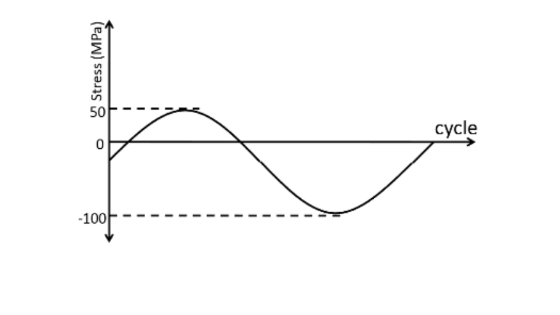
\includegraphics[width=0.5\linewidth]{figs/a5f3.png}
    \caption{}
    \label{fig:placeholder}
\end{figure}

For the above stress cycle:

\item Stress ratio is
\begin{multicols}{2}
\begin{enumerate}  
\item 4
\item 2
\item -2
\item -4
\end{enumerate}
\end{multicols}
\hfill(GATE MT 2012)

\item Amplitude ratio is
\begin{multicols}{2}
\begin{enumerate}  
\item 3
\item $1/3$
\item $-1/3$
\item -3
\end{enumerate}
\end{multicols}
\hfill(GATE MT 2012)

\item[] \textbf{Statement for Linked Answer Questions 52 and 53:} \\
A material with grain size of ASTM No. 6 has a lattice frictional stress 100 MN/m$^2$ and locking parameter (Hall-Petch constant) 0.10 MN/m$^{3/2}$

\item Grain size of the material is approximately
\begin{multicols}{2}
\begin{enumerate}  
\item 45 $\mu$m
\item 35 $\mu$m
\item 4.5 $\mu$m
\item 3.5 $\mu$m
\end{enumerate}
\end{multicols}
\hfill(GATE MT 2012)

\item Yield strength of the material is approximately
\begin{multicols}{2}
\begin{enumerate}  
\item 100 MPa
\item 115 MPa
\item 165 MPa
\item 215 MPa
\end{enumerate}
\end{multicols}
\hfill(GATE MT 2012)

\item[] \textbf{Statement for Linked Answer Questions 54 and 55:}\\
The strain hardening behaviour of an annealed rod during cold rolling is given by $\overline{\sigma} = 700(\epsilon)^{0.2}$ MPa, where $\overline{\sigma}$ is the flow stress at strain $\epsilon$.

\item Flow stress after $50\%$ reduction in area of the annealed rod on cold rolling is approximately
\begin{multicols}{2}
\begin{enumerate}  
\item 750 MPa
\item 650 MPa
\item 609 MPa
\item 559 MPa
\end{enumerate}
\end{multicols}
\hfill(GATE MT 2012)

\item If a wire of 5 mm diameter is drawn from the above cold rolled rod of 10 mm diameter, the drawing stress, neglecting the effect of friction and redundant work, is approximately
\begin{multicols}{2}
\begin{enumerate}  
\item 650 MPa
\item 550 MPa
\item 450 MPa
\item 400 MPa
\end{enumerate}
\end{multicols}
\hfill(GATE MT 2012)

\item Which one of the following options is the closest in meaning to the word given below?\\[0.5em]
\textbf{Latitude}
\begin{multicols}{2}
\begin{enumerate}  
\item Eligibility
\item Freedom
\item Coercion
\item Meticulousness
\end{enumerate}
\end{multicols}
\hfill(GATE MT 2012)

\item Choose the most appropriate word from the options given below to complete the following sentence:\\[0.5em]
\textbf{Given the seriousness of the situation that he had to face, his \_\_\_ was impressive.}
\begin{multicols}{2}
\begin{enumerate}  
\item beggary
\item nomenclature
\item jealousy
\item nonchalance
\end{enumerate}
\end{multicols}
\hfill(GATE MT 2012)

\item Choose the most appropriate alternative from the options given below to complete the following sentence:\\[0.5em]
\textbf{If the tired soldier wanted to lie down, he \_\_\_ the mattress out on the balcony.}
\begin{multicols}{2}
\begin{enumerate}  
\item should take
\item shall take
\item should have taken
\item will have taken
\end{enumerate}
\end{multicols}
\hfill(GATE MT 2012)

\item If $(1.001)^{1259} = 3.52$ and $ (1.001)^{2062} = 7.85 $, then $ (1.001)^{3321} = $
\begin{multicols}{2}
\begin{enumerate}  
\item 2.23
\item 4.33
\item 11.37
\item 27.64
\end{enumerate}
\end{multicols}
\hfill(GATE MT 2012)

\item One of the parts (A, B, C, D) in the sentence given below contains an \textbf{ERROR}. Which one of the following is \textbf{INCORRECT}?\\[0.5em]
\textbf{I requested that he should be given the driving test today instead of tomorrow.}
\begin{multicols}{2}
\begin{enumerate}  
\item requested that
\item should be given
\item the driving test
\item instead of tomorrow
\end{enumerate}
\end{multicols}
\hfill(GATE MT 2012)

\item The data given in the following table summarizes the monthly budget of an average household.
\[
    \begin{array}{|c|c|}
    \hline
    \text{Category} & \text{Amount (Rs.)} \\
    \hline
    \text{Food}        & 4000 \\
    \text{Clothing}    & 1200 \\
    \text{Rent}        & 2000 \\
    \text{Savings}     & 1500 \\
    \text{Other expenses} & 1800 \\
    \hline
    \end{array}
\]
The approximate percentage of the monthly budget \textbf{NOT} spent on savings is
\begin{multicols}{2}
\begin{enumerate}  
\item 10\%
\item 14\%
\item 81\%
\item 86\%
\end{enumerate}
\end{multicols}
\hfill(GATE MT 2012)

\item There are eight bags of rice looking alike, seven of which have equal weight and one is slightly heavier. The weighing balance is of unlimited capacity. Using this balance, the minimum number of weighings required to identify the heavier bag is
\begin{multicols}{2}
\begin{enumerate}  
\item 2
\item 3
\item 4
\item 8
\end{enumerate}
\end{multicols}
\hfill(GATE MT 2012)

\item Raju has 14 currency notes in his pocket consisting of only Rs. 20 notes and Rs. 10 notes. The total money value of the notes is Rs. 230. The number of Rs. 10 notes that Raju has is
\begin{multicols}{2}
\begin{enumerate}  
\item 5
\item 6
\item 9
\item 10
\end{enumerate}
\end{multicols}
\hfill(GATE MT 2012)

\item One of the legacies of the Roman legions was discipline. In the legions, military law prevailed and discipline was brutal. Discipline on the battlefield kept units obedient, intact and fighting, even when the odds and conditions were against them.
Which one of the following statements best sums up the meaning of the above passage?
\begin{multicols}{2}
\begin{enumerate}  
\item Thorough regimentation was the main reason for the efficiency of the Roman legions even in adverse circumstances.
\item The legions were treated inhumanly as if the men were animals.
\item Discipline was the armies' inheritance from their seniors.
\item The harsh discipline to which the legions were subjected to led to the odds and conditions being against them.
\end{enumerate}
\end{multicols}
\hfill(GATE MT 2012)

\item A and B are friends. They decide to meet between 1 PM and 2 PM on a given day. There is a condition that whoever arrives first will not wait for the other for more than 15 minutes. The probability that they will meet on that day is
\begin{multicols}{2}
\begin{enumerate}  
\item $1/4$
\item $1/16$
\item $7/16$
\item $9/16$
\end{enumerate}
\end{multicols}
\hfill(GATE MT 2012)

\end{enumerate}



\begin{center}
\textbf{END OF THE QUESTION PAPER}
\end{center}

\end{document}